\documentclass[12pt, a4paper]{article}

\usepackage{graphicx}
\usepackage{float}
\usepackage{subfloat}
\usepackage{subfig}
\usepackage[left=.75in,top=.75in,right=.75in,bottom=.75in]{geometry}

\begin{document} 

\section{Plots based on (binary) function overlap}
\subsection{Rat}
\begin{figure}[H]
\caption{Plots based on original dataset}
\centerline{
\subfloat[DSD vs Density]{
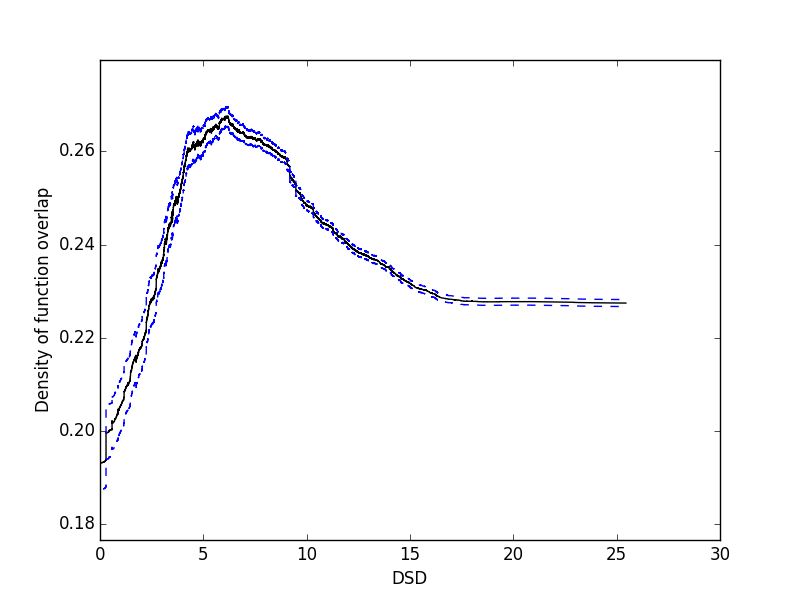
\includegraphics[width=0.333333333333\textwidth]{plots/rat_dsd_density.png}
}
\subfloat[DSD vs Overlap, Pairs]{
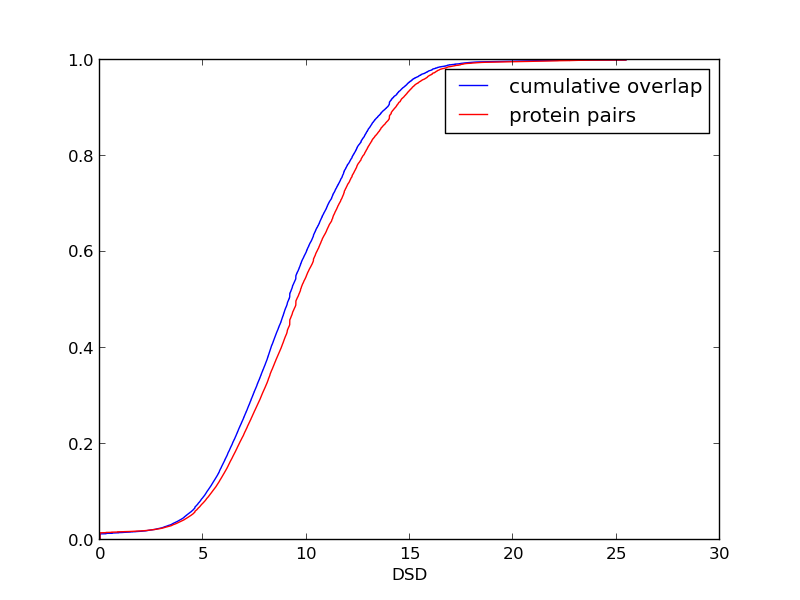
\includegraphics[width=0.333333333333\textwidth]{plots/rat_dsd_overlap_pairs.png}
}
\subfloat[Pairs vs Cumulative Overlap]{
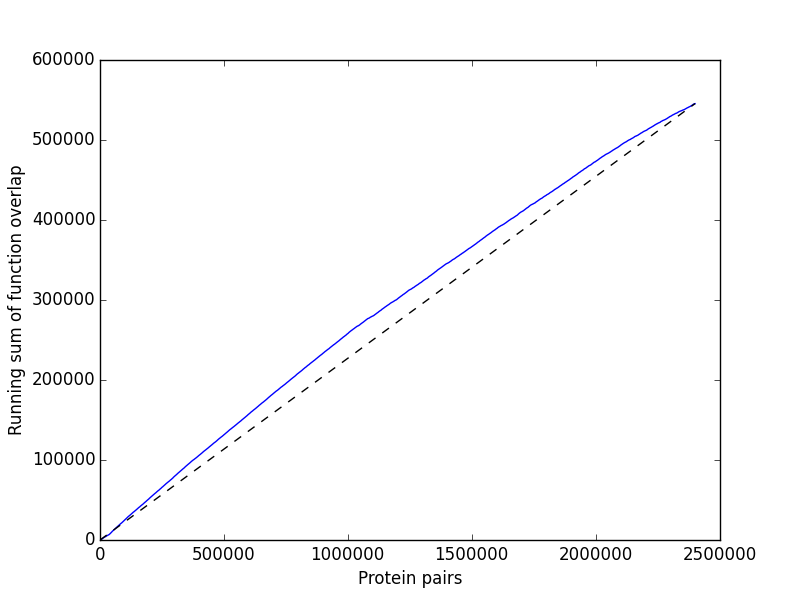
\includegraphics[width=0.333333333333\textwidth]{plots/rat_pairs_overlap.png}
}
}
\end{figure}

\begin{figure}[H]
\caption{Plots based on random permutation of label sets}
\centerline{
\subfloat[DSD vs Density]{
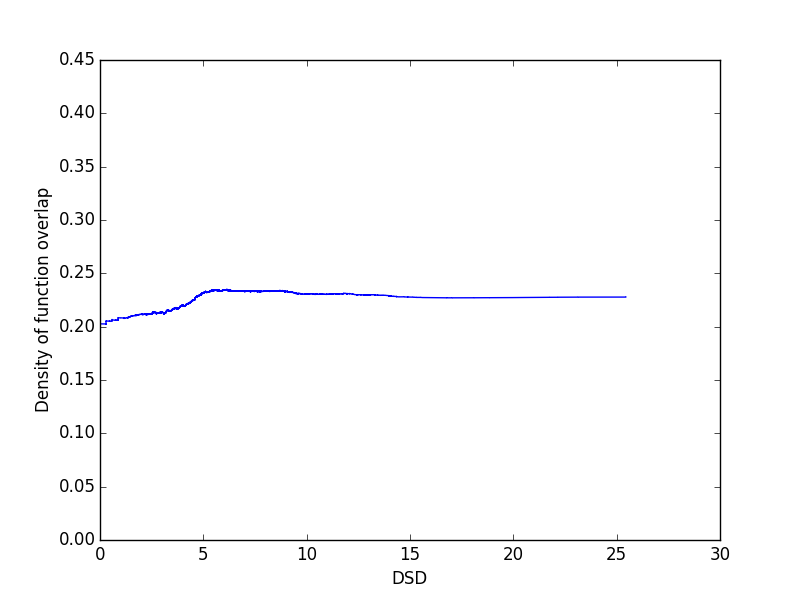
\includegraphics[width=0.333333333333\textwidth]{plots/rat_dsd_density_randomized.png}
}
\subfloat[DSD vs Overlap, Pairs]{
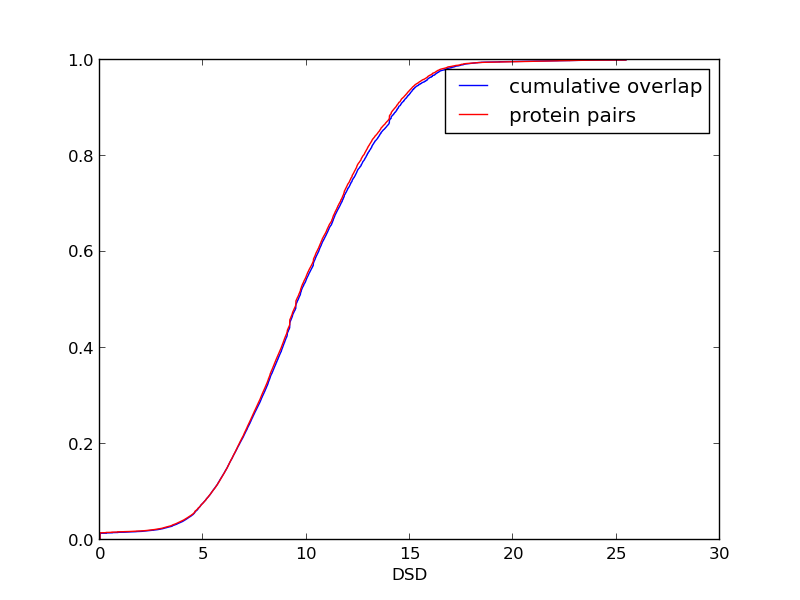
\includegraphics[width=0.333333333333\textwidth]{plots/rat_dsd_overlap_pairs_randomized.png}
}
\subfloat[Pairs vs Cumulative Overlap]{
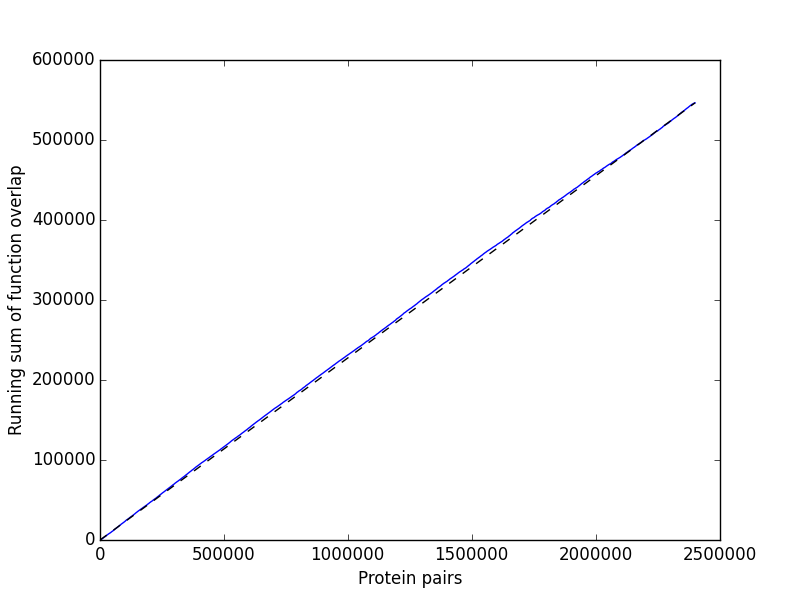
\includegraphics[width=0.333333333333\textwidth]{plots/rat_pairs_overlap_randomized.png}
}
}
\end{figure}

\begin{figure}[H]
\caption{Shortest-path distance (SPD) comparisons}
\centerline{
\subfloat[SPD vs Density]{
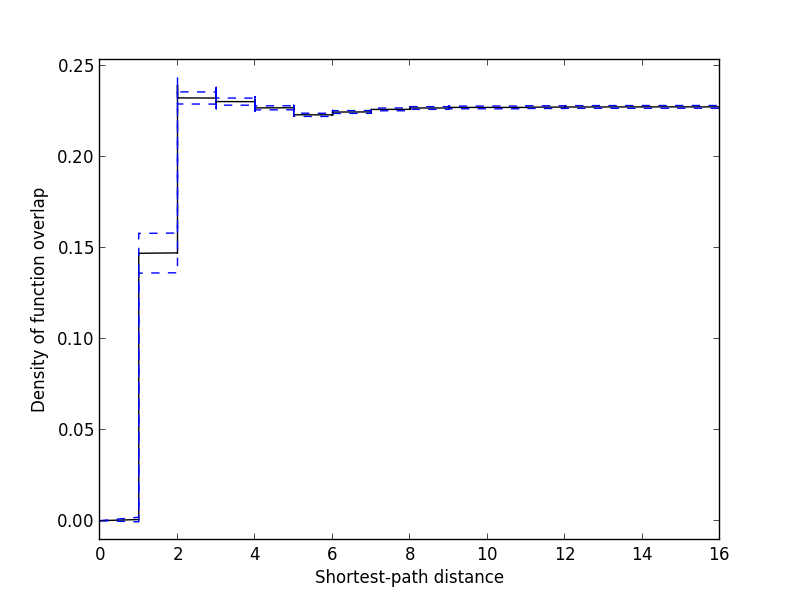
\includegraphics[width=0.333333333333\textwidth]{plots/rat_spd_density.png}
}
\subfloat[SPD vs Overlap, Pairs]{
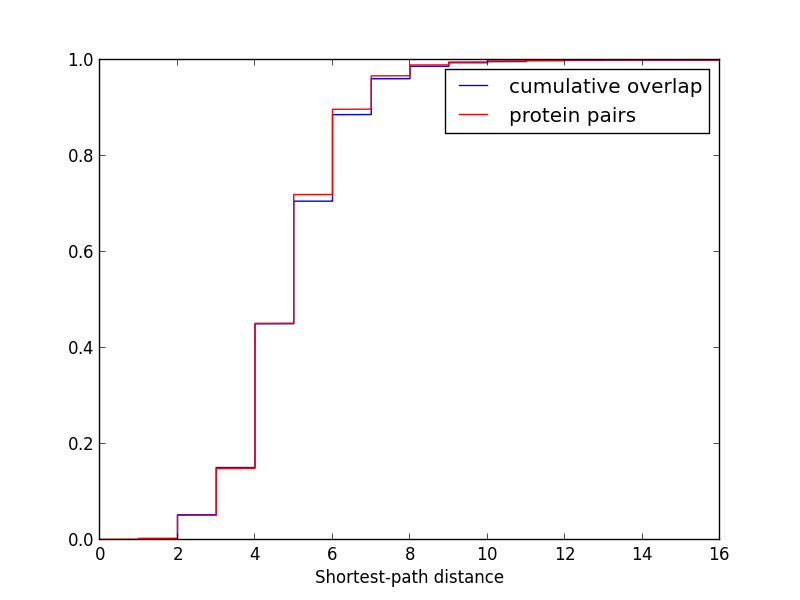
\includegraphics[width=0.333333333333\textwidth]{plots/rat_spd_overlap_pairs.png}
}
}
\end{figure}

\subsection{Worm}
\begin{figure}[H]
\caption{Plots based on original dataset}
\centerline{
\subfloat[DSD vs Density]{
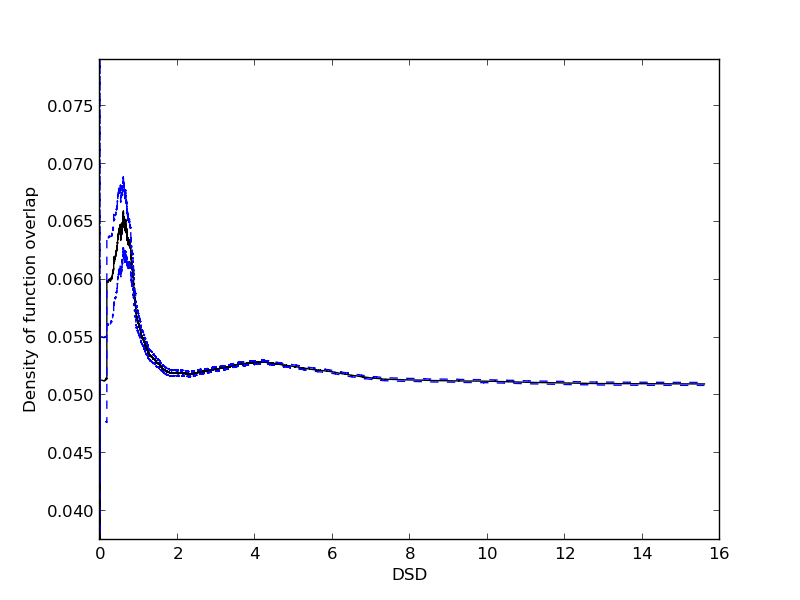
\includegraphics[width=0.333333333333\textwidth]{plots/worm_dsd_density.png}
}
\subfloat[DSD vs Overlap, Pairs]{
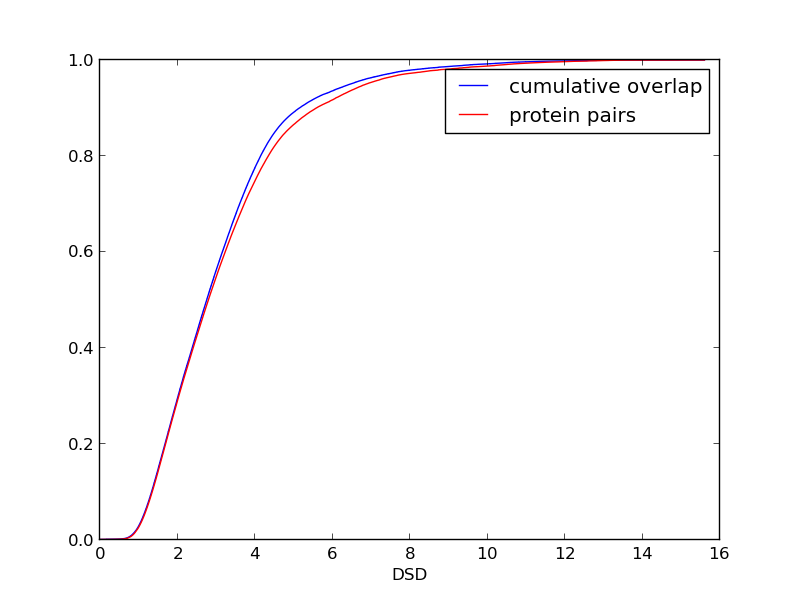
\includegraphics[width=0.333333333333\textwidth]{plots/worm_dsd_overlap_pairs.png}
}
\subfloat[Pairs vs Cumulative Overlap]{
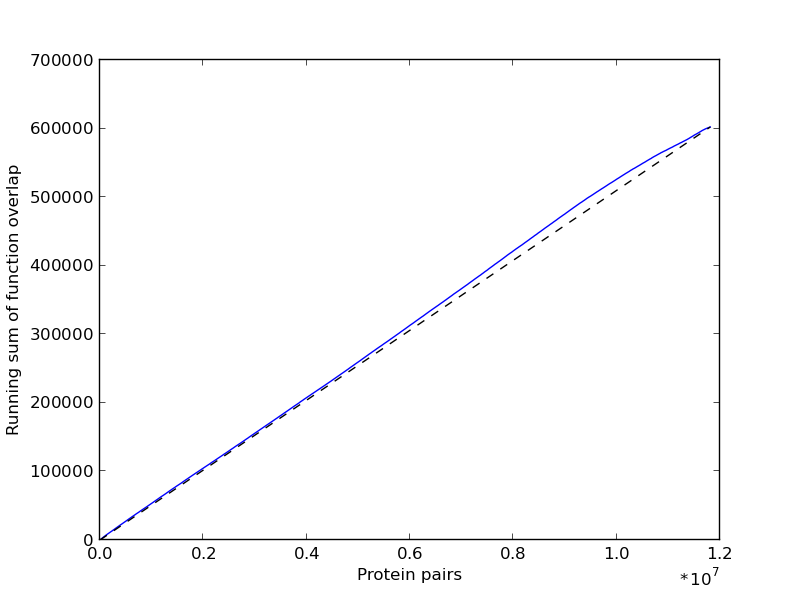
\includegraphics[width=0.333333333333\textwidth]{plots/worm_pairs_overlap.png}
}
}
\end{figure}

\begin{figure}[H]
\caption{Plots based on random permutation of label sets}
\centerline{
\subfloat[DSD vs Density]{
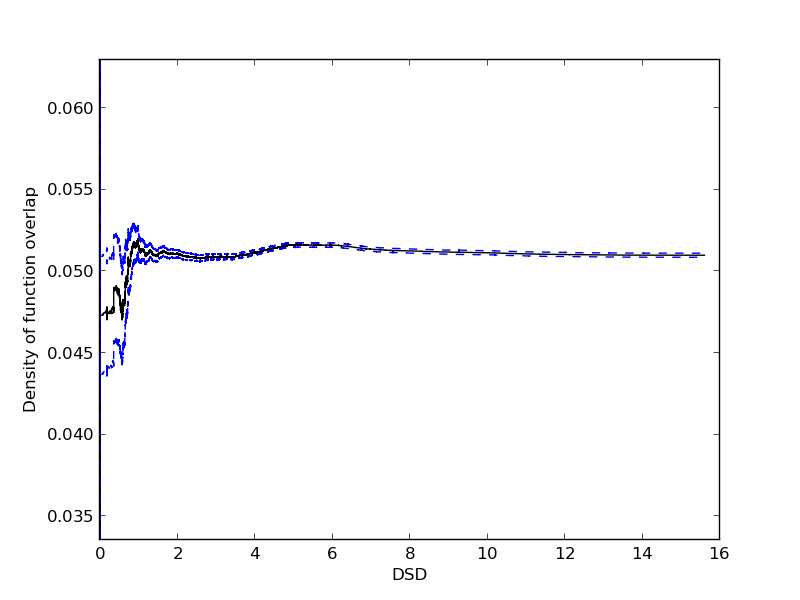
\includegraphics[width=0.333333333333\textwidth]{plots/worm_dsd_density_randomized.png}
}
\subfloat[DSD vs Overlap, Pairs]{
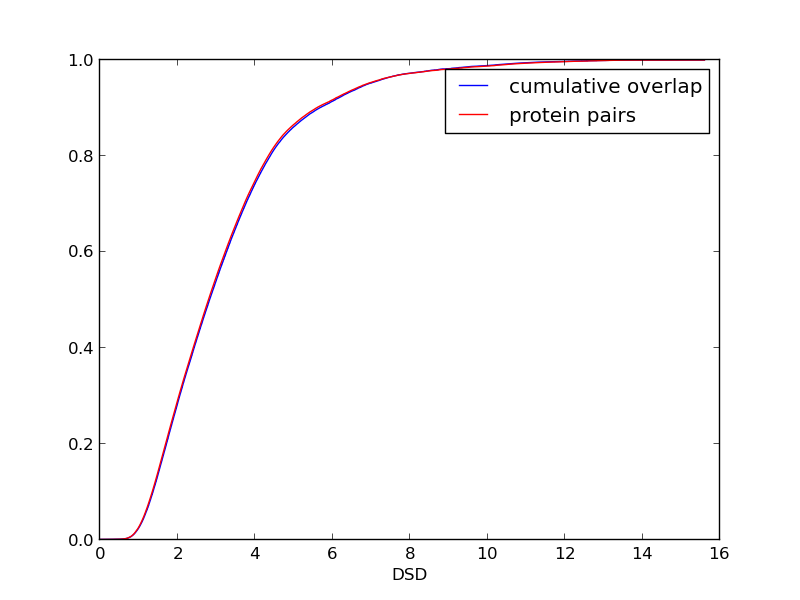
\includegraphics[width=0.333333333333\textwidth]{plots/worm_dsd_overlap_pairs_randomized.png}
}
\subfloat[Pairs vs Cumulative Overlap]{
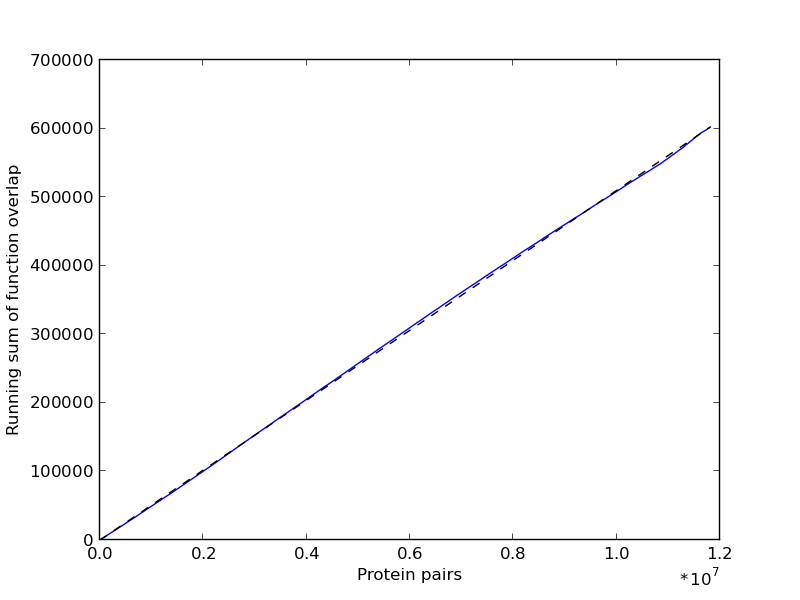
\includegraphics[width=0.333333333333\textwidth]{plots/worm_pairs_overlap_randomized.png}
}
}
\end{figure}

\begin{figure}[H]
\caption{Shortest-path distance (SPD) comparisons}
\centerline{
\subfloat[SPD vs Density]{
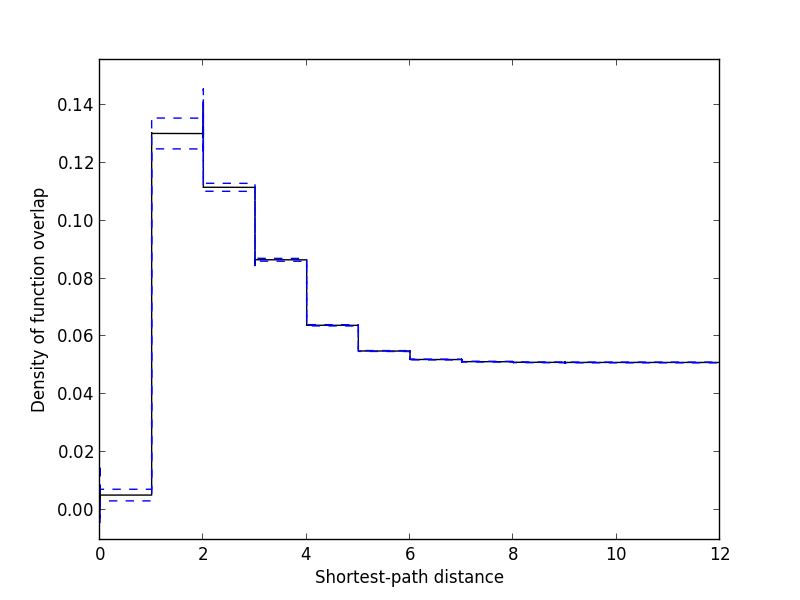
\includegraphics[width=0.333333333333\textwidth]{plots/worm_spd_density.png}
}
\subfloat[SPD vs Overlap, Pairs]{
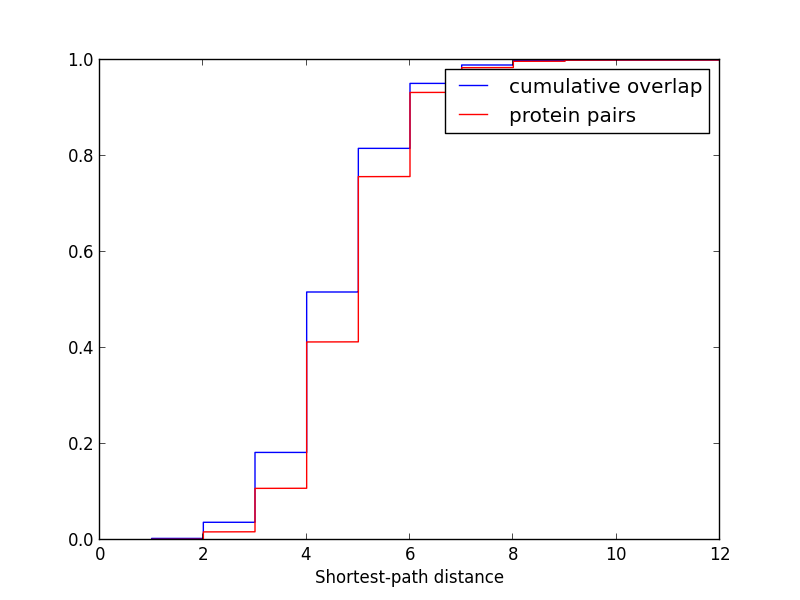
\includegraphics[width=0.333333333333\textwidth]{plots/worm_spd_overlap_pairs.png}
}
}
\end{figure}

\subsection{Mouse}
\begin{figure}[H]
\caption{Plots based on original dataset}
\centerline{
\subfloat[DSD vs Density]{
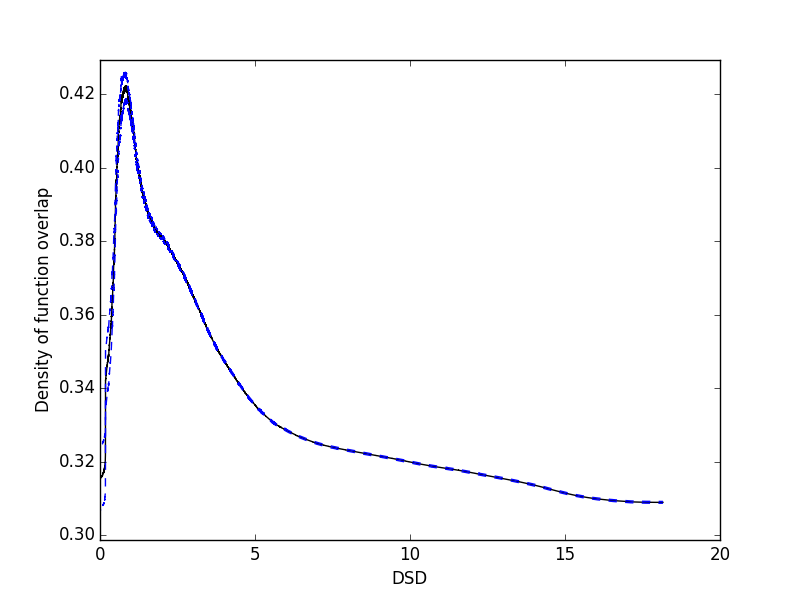
\includegraphics[width=0.333333333333\textwidth]{plots/mouse_dsd_density.png}
}
\subfloat[DSD vs Overlap, Pairs]{
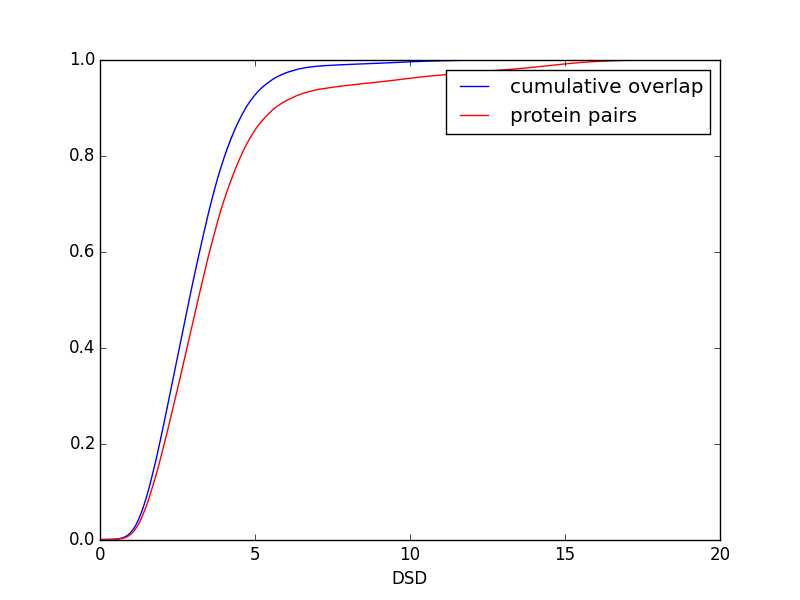
\includegraphics[width=0.333333333333\textwidth]{plots/mouse_dsd_overlap_pairs.png}
}
\subfloat[Pairs vs Cumulative Overlap]{
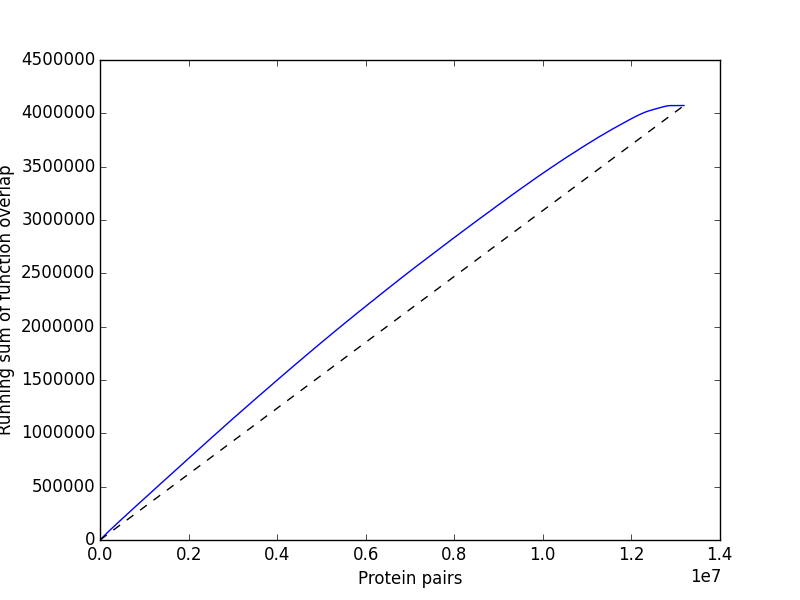
\includegraphics[width=0.333333333333\textwidth]{plots/mouse_pairs_overlap.png}
}
}
\end{figure}

\begin{figure}[H]
\caption{Plots based on random permutation of label sets}
\centerline{
\subfloat[DSD vs Density]{
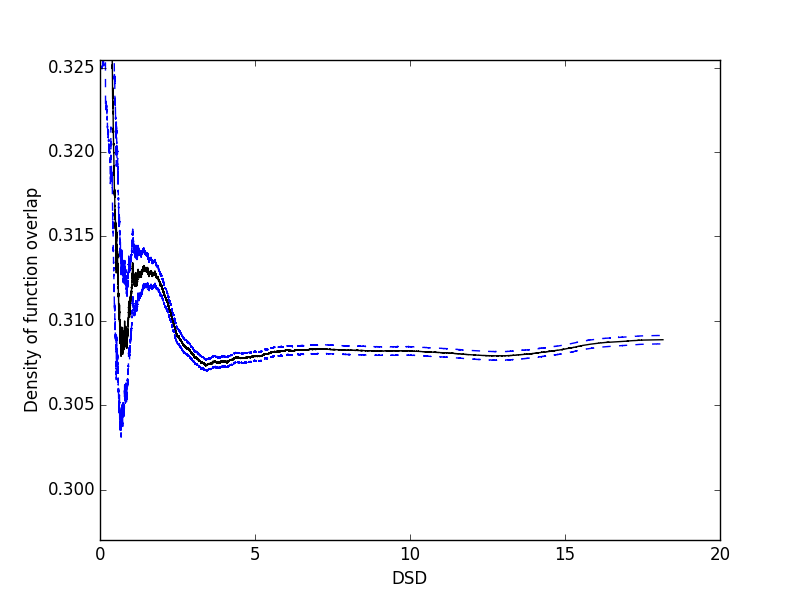
\includegraphics[width=0.333333333333\textwidth]{plots/mouse_dsd_density_randomized.png}
}
\subfloat[DSD vs Overlap, Pairs]{
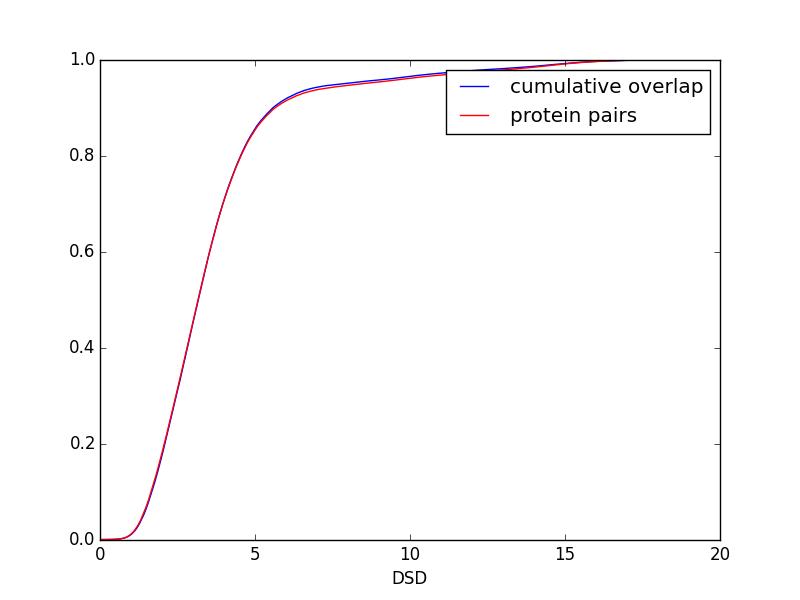
\includegraphics[width=0.333333333333\textwidth]{plots/mouse_dsd_overlap_pairs_randomized.png}
}
\subfloat[Pairs vs Cumulative Overlap]{
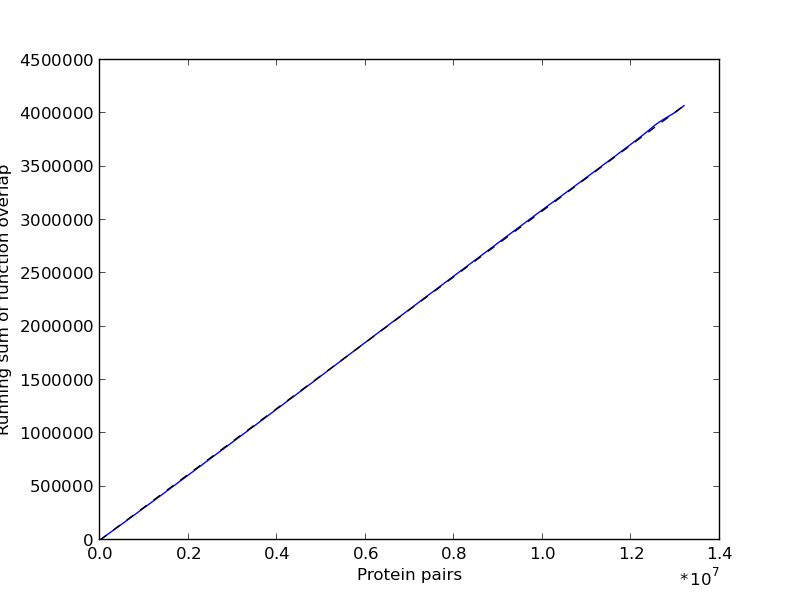
\includegraphics[width=0.333333333333\textwidth]{plots/mouse_pairs_overlap_randomized.png}
}
}
\end{figure}

\begin{figure}[H]
\caption{Shortest-path distance (SPD) comparisons}
\centerline{
\subfloat[SPD vs Density]{
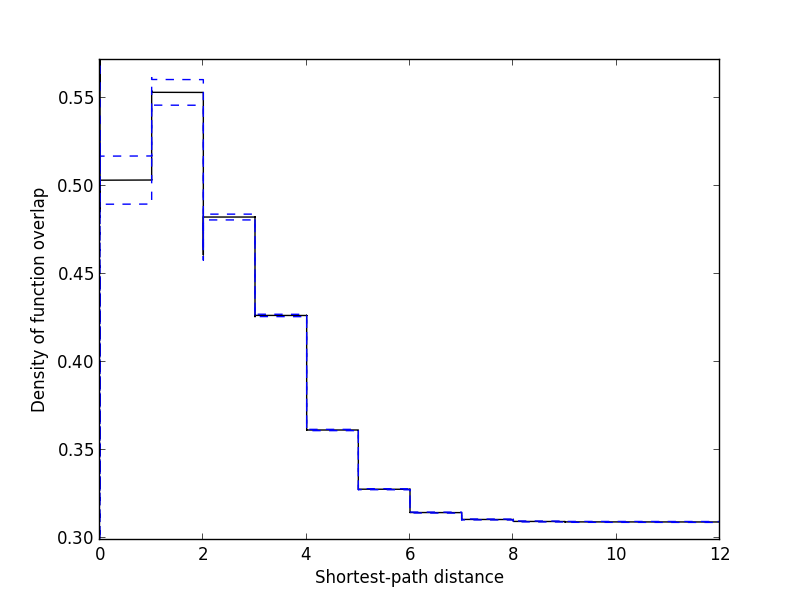
\includegraphics[width=0.333333333333\textwidth]{plots/mouse_spd_density.png}
}
\subfloat[SPD vs Overlap, Pairs]{
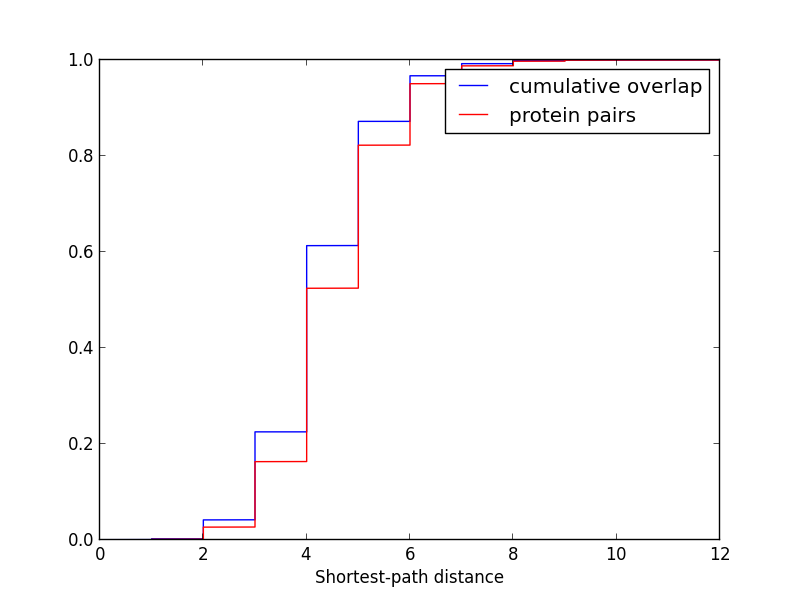
\includegraphics[width=0.333333333333\textwidth]{plots/mouse_spd_overlap_pairs.png}
}
}
\end{figure}

\subsection{Fly}
\begin{figure}[H]
\caption{Plots based on original dataset}
\centerline{
\subfloat[DSD vs Density]{
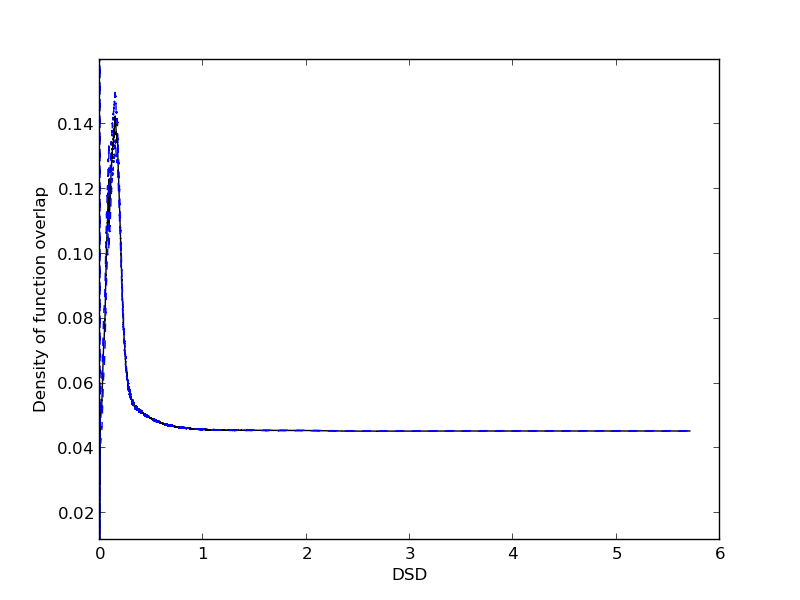
\includegraphics[width=0.333333333333\textwidth]{plots/fly_dsd_density.png}
}
\subfloat[DSD vs Overlap, Pairs]{
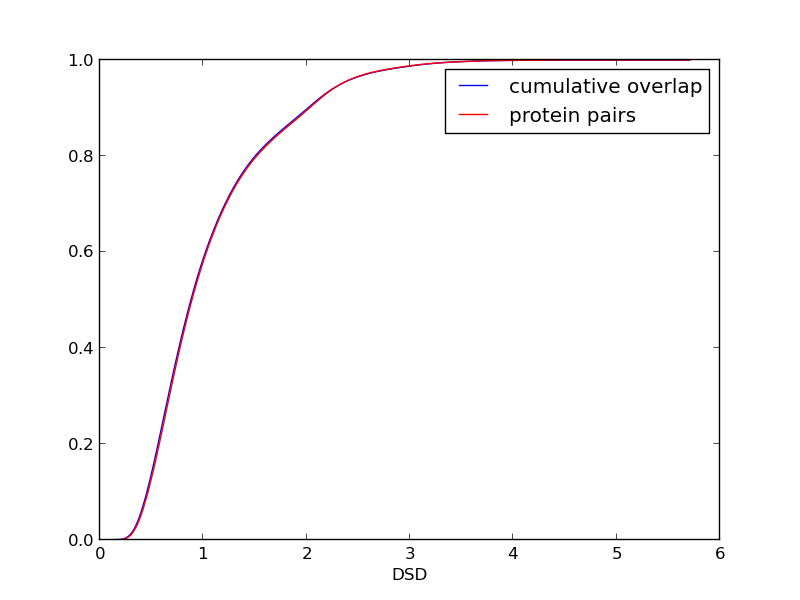
\includegraphics[width=0.333333333333\textwidth]{plots/fly_dsd_overlap_pairs.png}
}
\subfloat[Pairs vs Cumulative Overlap]{
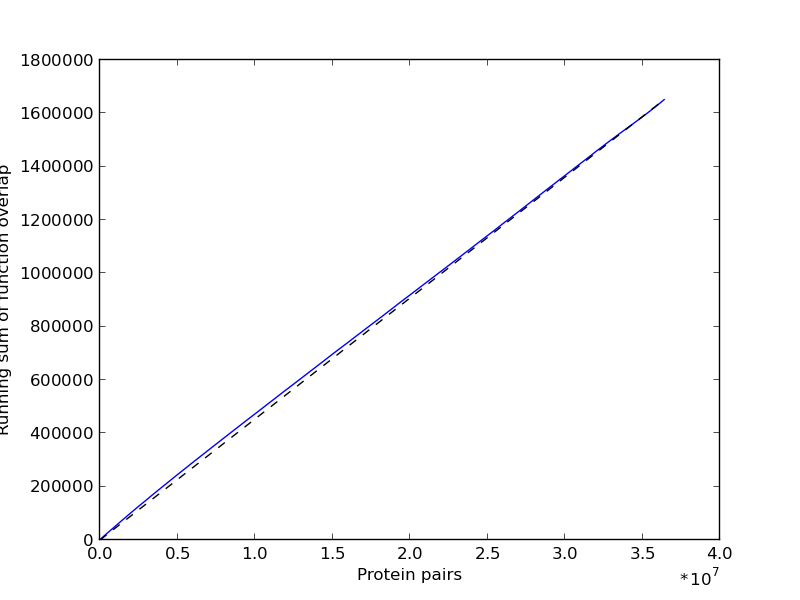
\includegraphics[width=0.333333333333\textwidth]{plots/fly_pairs_overlap.png}
}
}
\end{figure}

\begin{figure}[H]
\caption{Plots based on random permutation of label sets}
\centerline{
\subfloat[DSD vs Density]{
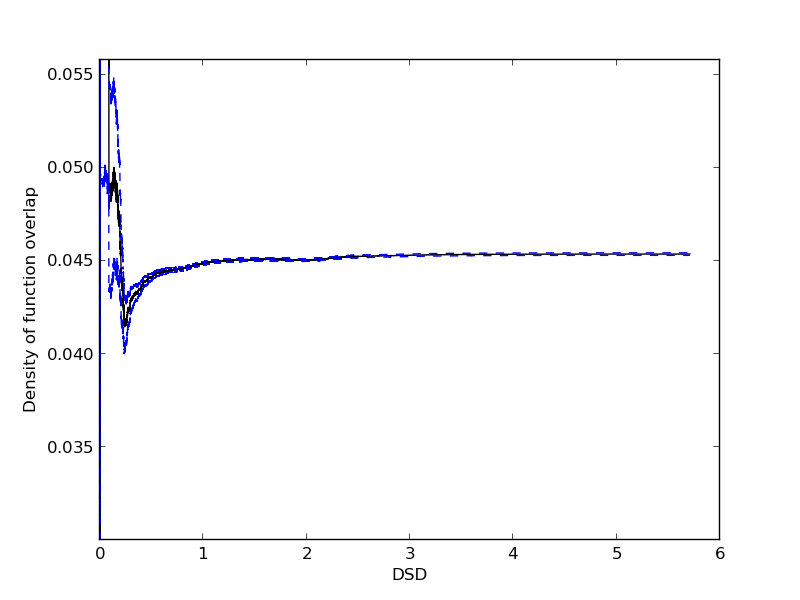
\includegraphics[width=0.333333333333\textwidth]{plots/fly_dsd_density_randomized.png}
}
\subfloat[DSD vs Overlap, Pairs]{
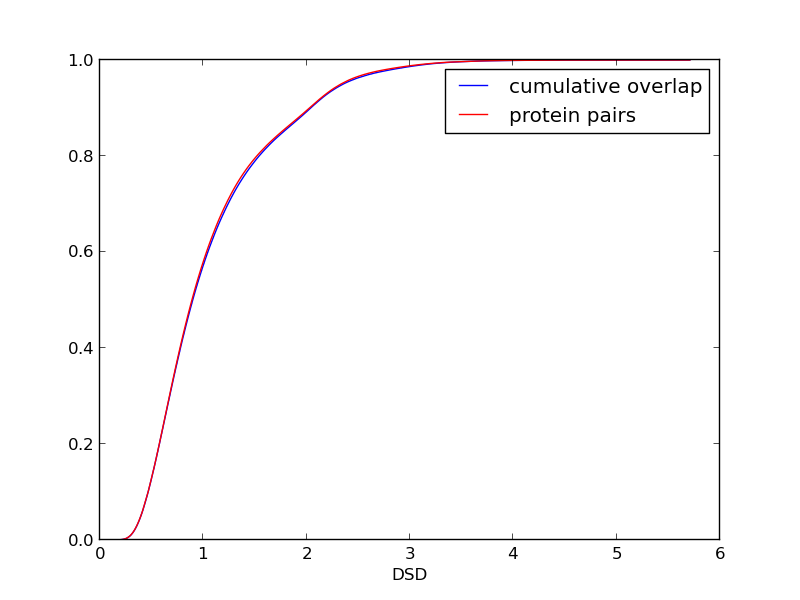
\includegraphics[width=0.333333333333\textwidth]{plots/fly_dsd_overlap_pairs_randomized.png}
}
\subfloat[Pairs vs Cumulative Overlap]{
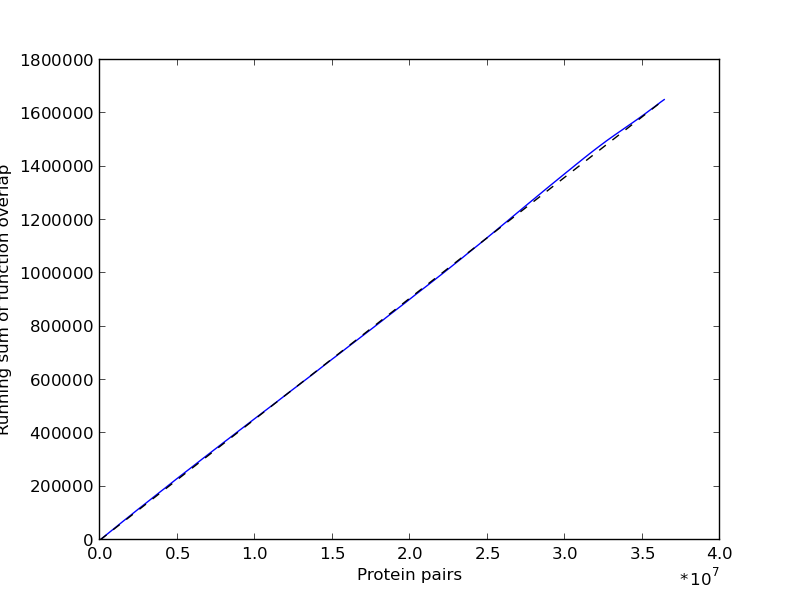
\includegraphics[width=0.333333333333\textwidth]{plots/fly_pairs_overlap_randomized.png}
}
}
\end{figure}

\begin{figure}[H]
\caption{Shortest-path distance (SPD) comparisons}
\centerline{
\subfloat[SPD vs Density]{
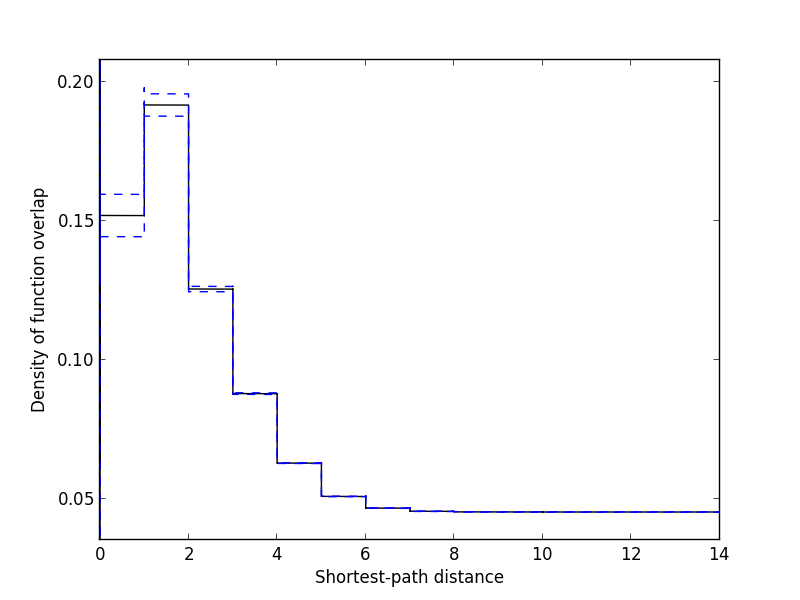
\includegraphics[width=0.333333333333\textwidth]{plots/fly_spd_density.png}
}
\subfloat[SPD vs Overlap, Pairs]{
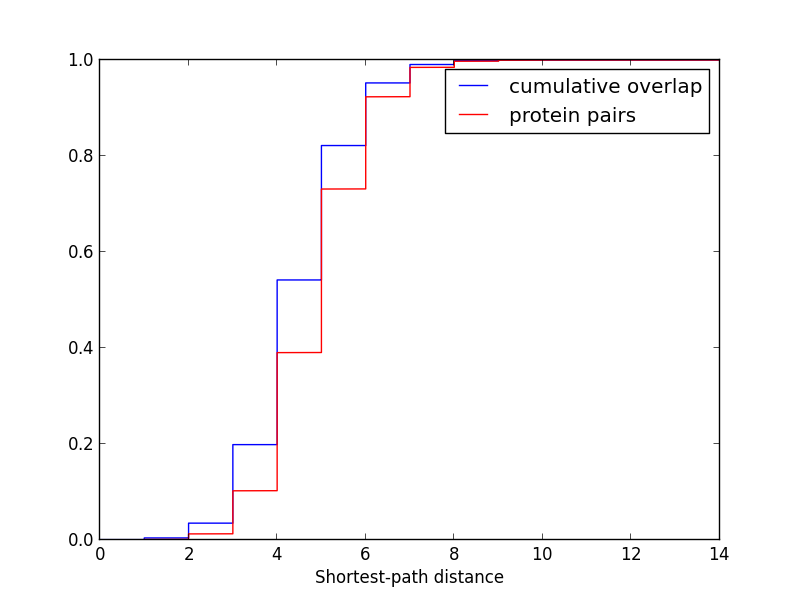
\includegraphics[width=0.333333333333\textwidth]{plots/fly_spd_overlap_pairs.png}
}
}
\end{figure}

\subsection{Human}
\begin{figure}[H]
\caption{Plots based on original dataset}
\centerline{
\subfloat[DSD vs Density]{
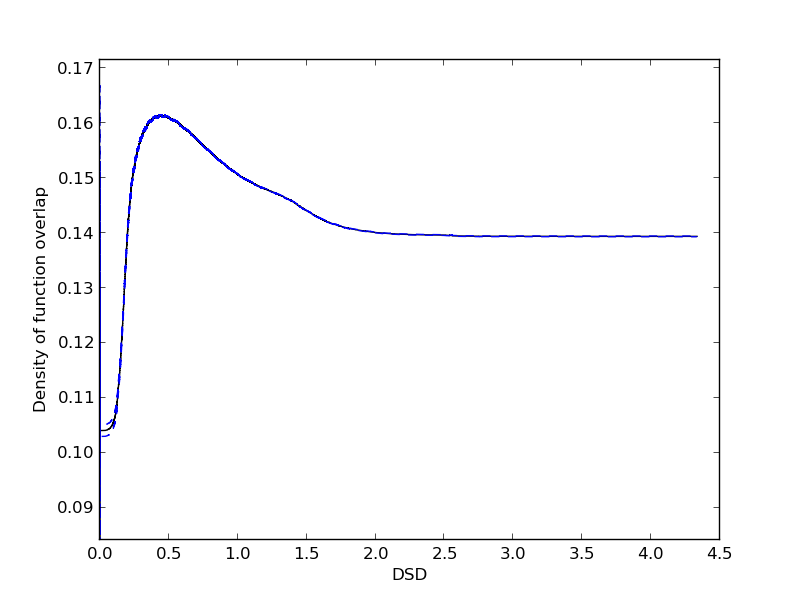
\includegraphics[width=0.333333333333\textwidth]{plots/human_dsd_density.png}
}
\subfloat[DSD vs Overlap, Pairs]{
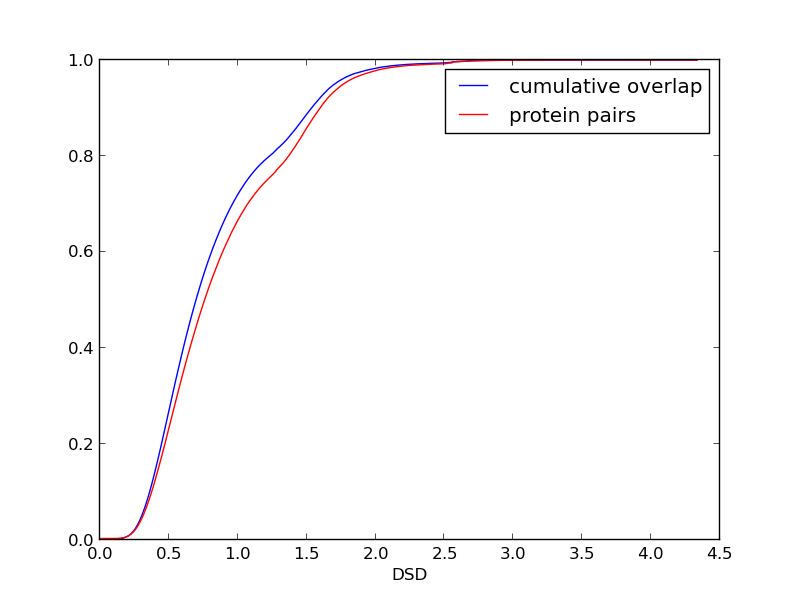
\includegraphics[width=0.333333333333\textwidth]{plots/human_dsd_overlap_pairs.png}
}
\subfloat[Pairs vs Cumulative Overlap]{
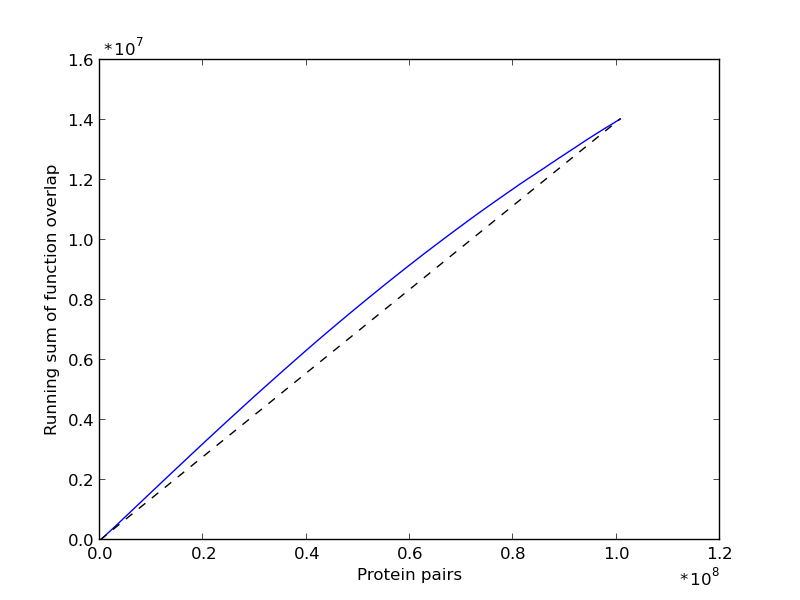
\includegraphics[width=0.333333333333\textwidth]{plots/human_pairs_overlap.png}
}
}
\end{figure}

\begin{figure}[H]
\caption{Plots based on random permutation of label sets}
\centerline{
\subfloat[DSD vs Density]{
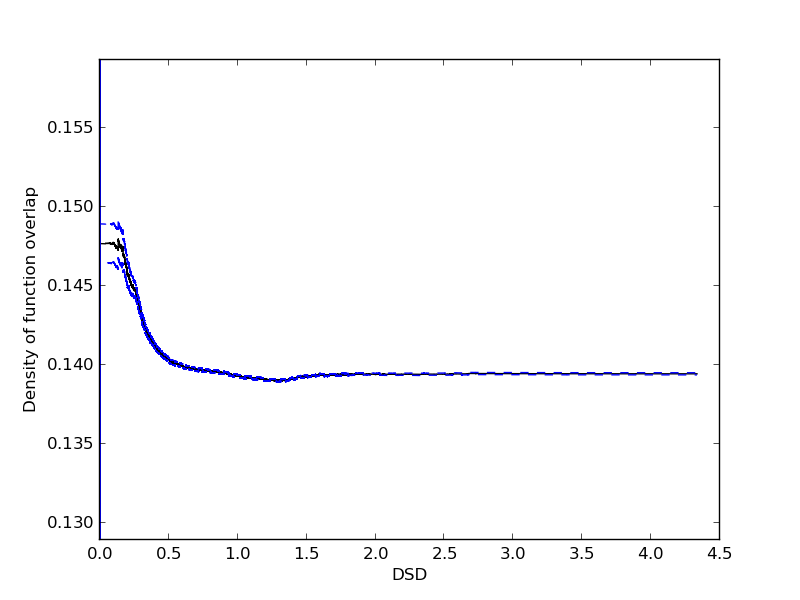
\includegraphics[width=0.333333333333\textwidth]{plots/human_dsd_density_randomized.png}
}
\subfloat[DSD vs Overlap, Pairs]{
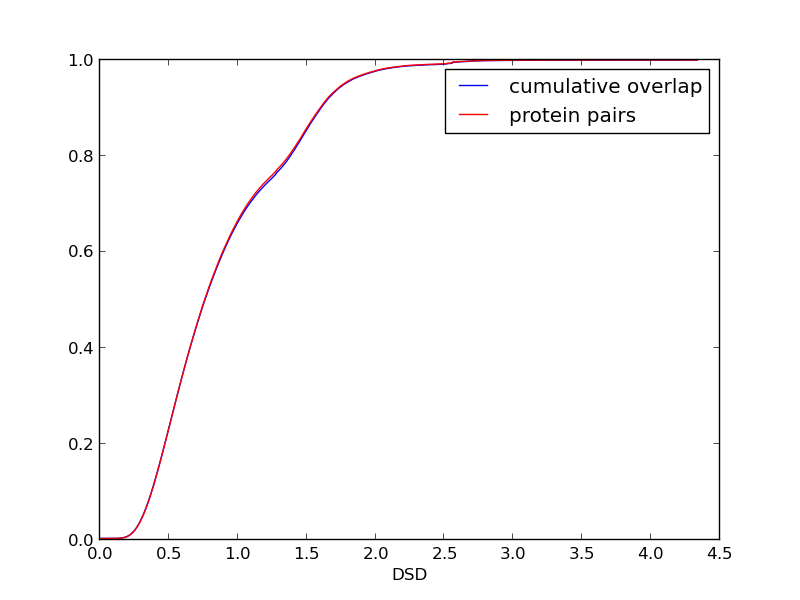
\includegraphics[width=0.333333333333\textwidth]{plots/human_dsd_overlap_pairs_randomized.png}
}
\subfloat[Pairs vs Cumulative Overlap]{
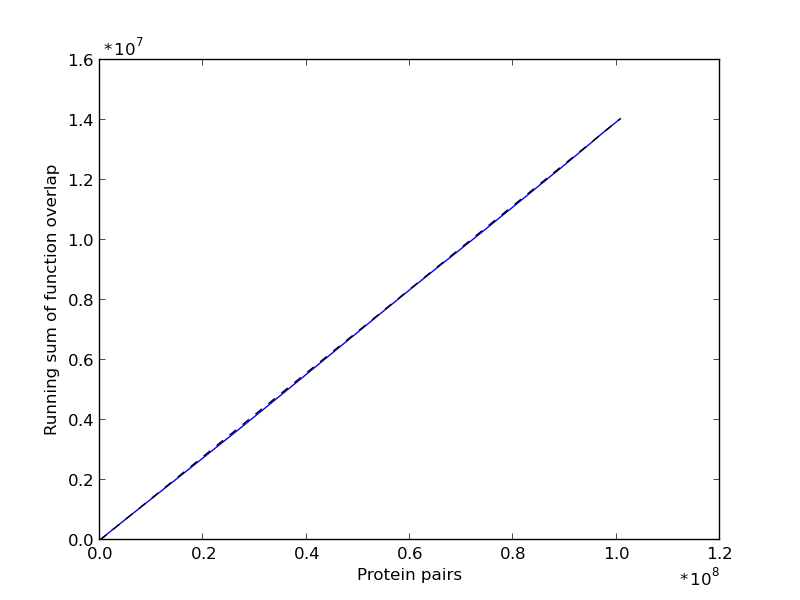
\includegraphics[width=0.333333333333\textwidth]{plots/human_pairs_overlap_randomized.png}
}
}
\end{figure}

\begin{figure}[H]
\caption{Shortest-path distance (SPD) comparisons}
\centerline{
\subfloat[SPD vs Density]{
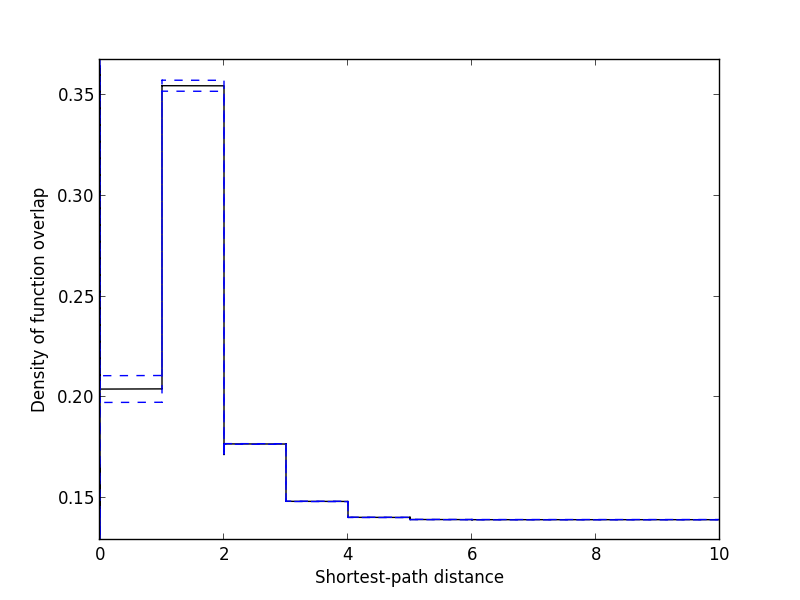
\includegraphics[width=0.333333333333\textwidth]{plots/human_spd_density.png}
}
\subfloat[SPD vs Overlap, Pairs]{
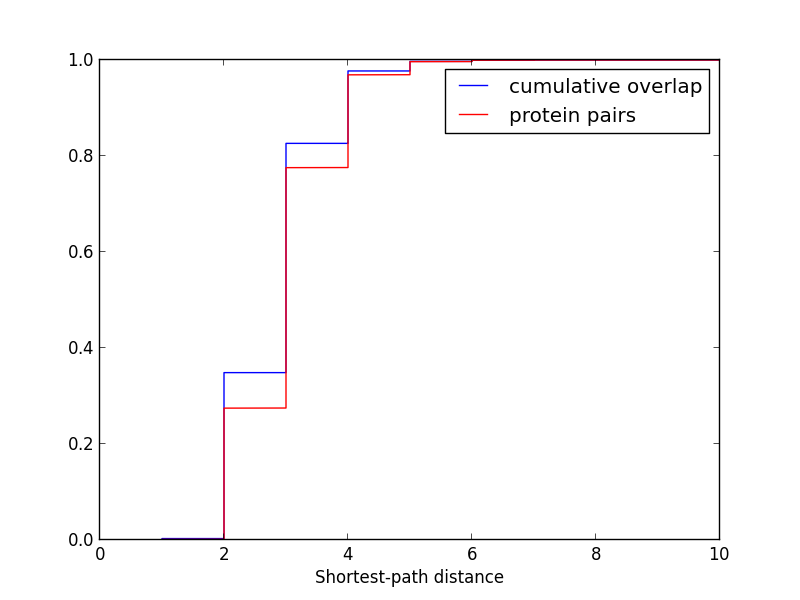
\includegraphics[width=0.333333333333\textwidth]{plots/human_spd_overlap_pairs.png}
}
}
\end{figure}

\subsection{Yeast}
\begin{figure}[H]
\caption{Plots based on original dataset}
\centerline{
\subfloat[DSD vs Density]{
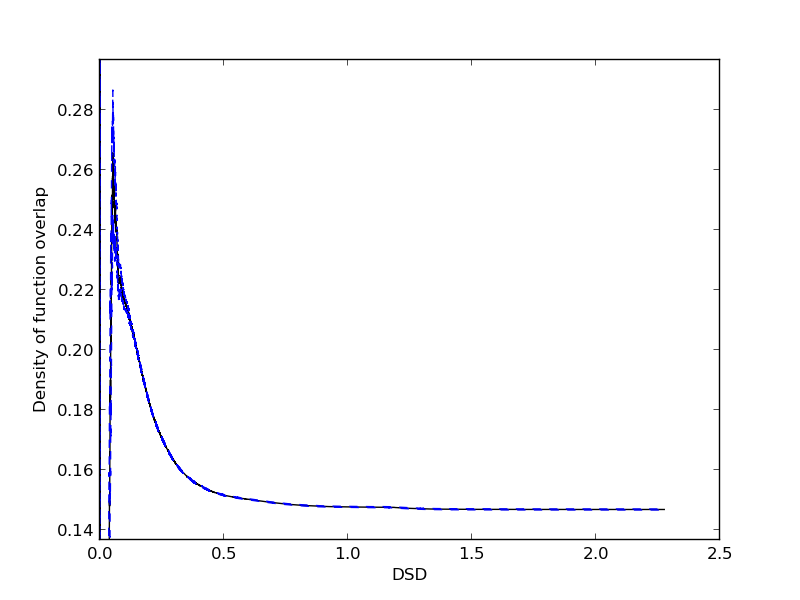
\includegraphics[width=0.333333333333\textwidth]{plots/yeast_dsd_density.png}
}
\subfloat[DSD vs Overlap, Pairs]{
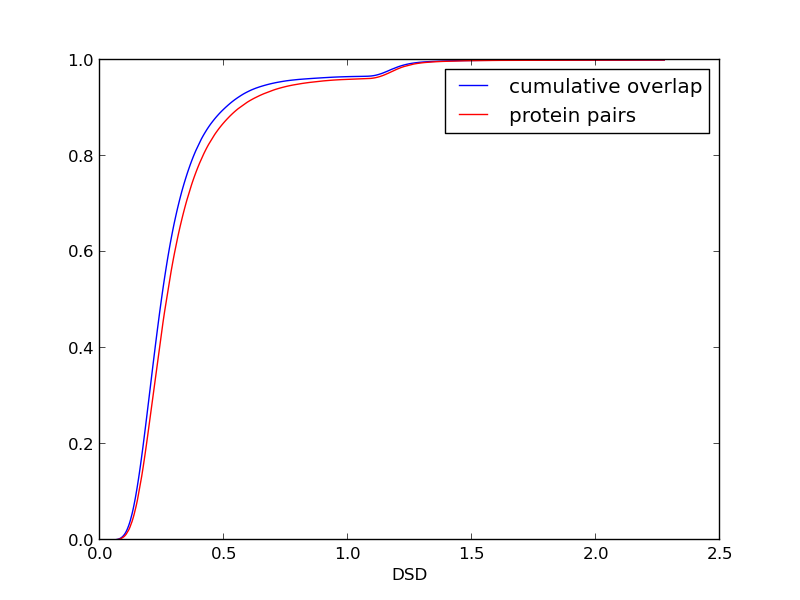
\includegraphics[width=0.333333333333\textwidth]{plots/yeast_dsd_overlap_pairs.png}
}
\subfloat[Pairs vs Cumulative Overlap]{
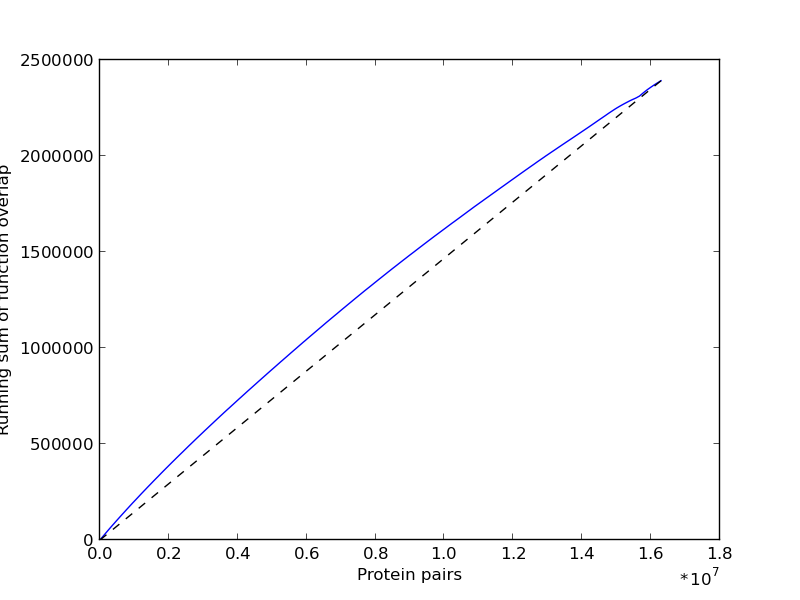
\includegraphics[width=0.333333333333\textwidth]{plots/yeast_pairs_overlap.png}
}
}
\end{figure}

\begin{figure}[H]
\caption{Plots based on random permutation of label sets}
\centerline{
\subfloat[DSD vs Density]{
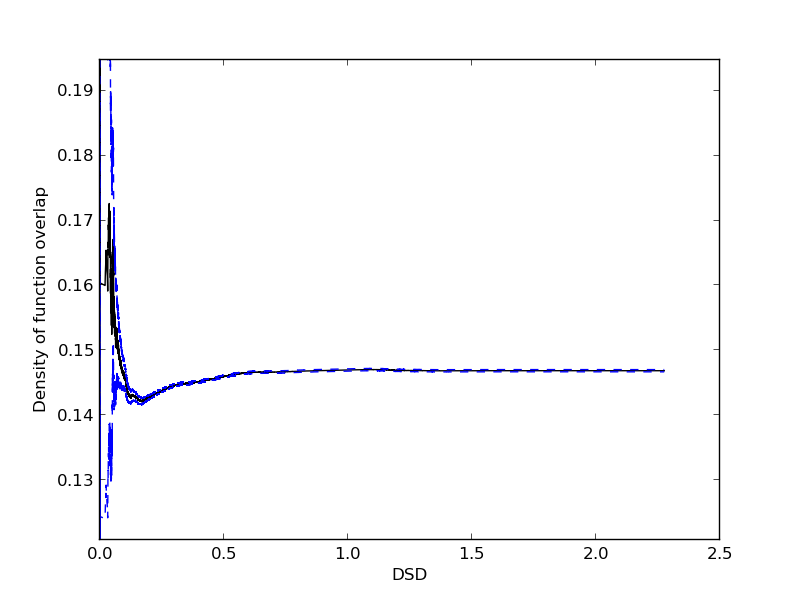
\includegraphics[width=0.333333333333\textwidth]{plots/yeast_dsd_density_randomized.png}
}
\subfloat[DSD vs Overlap, Pairs]{
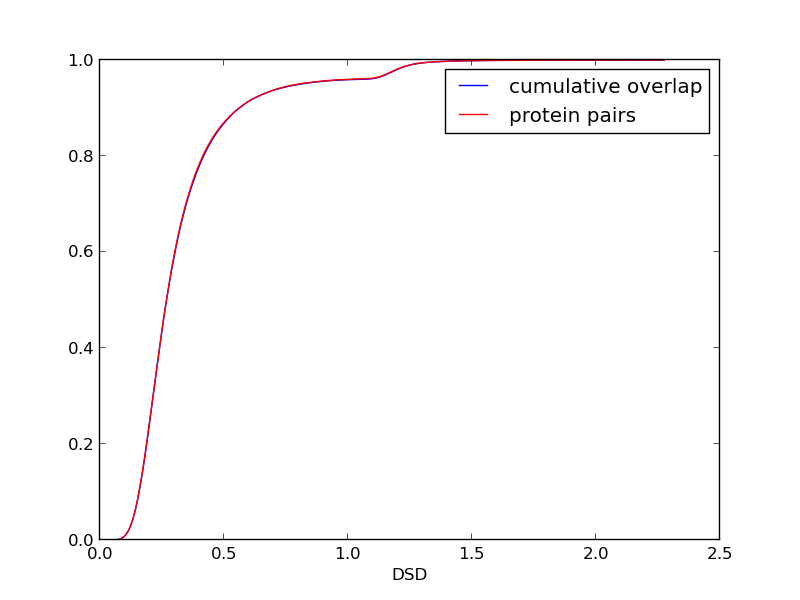
\includegraphics[width=0.333333333333\textwidth]{plots/yeast_dsd_overlap_pairs_randomized.png}
}
\subfloat[Pairs vs Cumulative Overlap]{
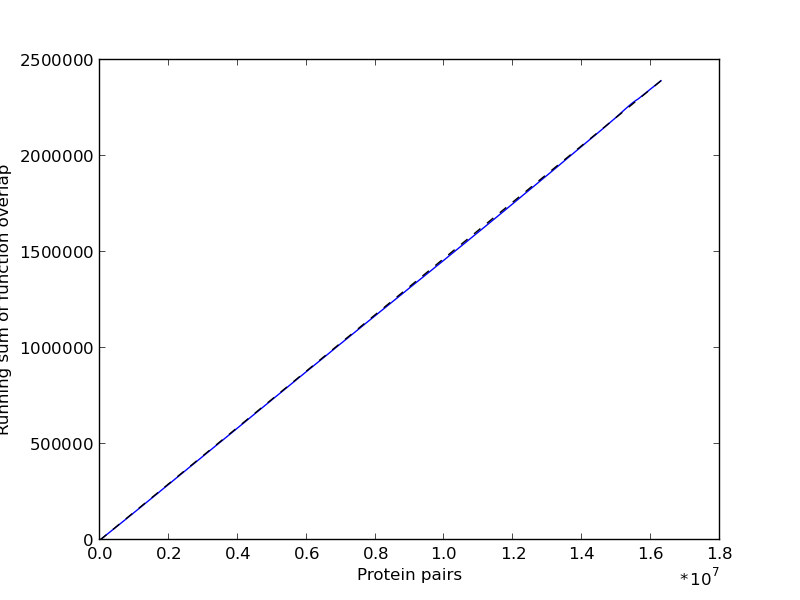
\includegraphics[width=0.333333333333\textwidth]{plots/yeast_pairs_overlap_randomized.png}
}
}
\end{figure}

\begin{figure}[H]
\caption{Shortest-path distance (SPD) comparisons}
\centerline{
\subfloat[SPD vs Density]{
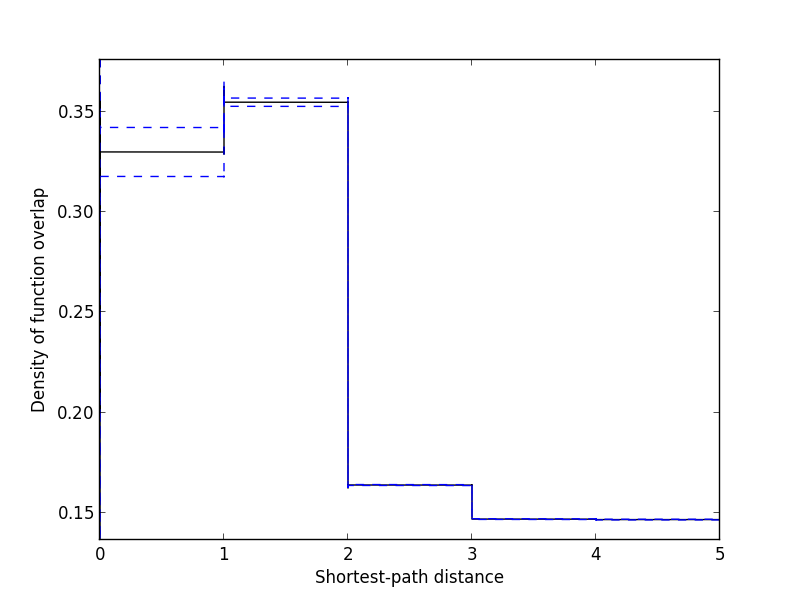
\includegraphics[width=0.333333333333\textwidth]{plots/yeast_spd_density.png}
}
\subfloat[SPD vs Overlap, Pairs]{
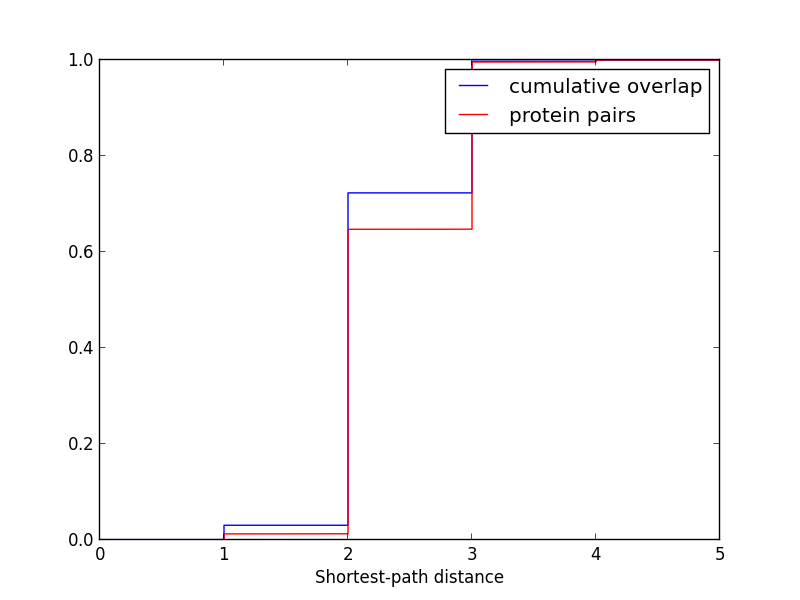
\includegraphics[width=0.333333333333\textwidth]{plots/yeast_spd_overlap_pairs.png}
}
}
\end{figure}

\section{Sorted pairs vs density plots}
\begin{figure}[H]
\caption{DSD only, with varying landmark set sizes}
\centerline{
\subfloat[Rat]{
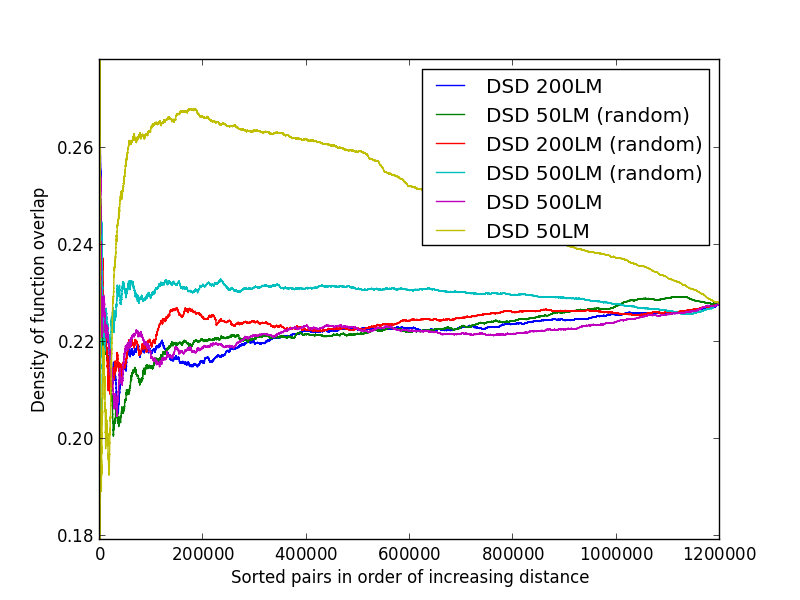
\includegraphics[width=0.333333333333\textwidth]{plots/sorted_pairs/dsd50_dsd200_dsd500/rat_alld_pairs_density.png}
}
\subfloat[Mouse]{
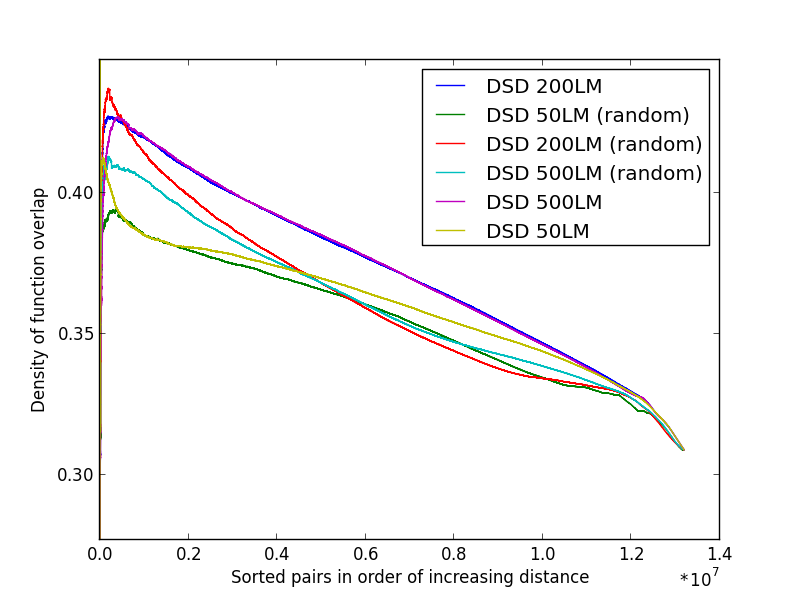
\includegraphics[width=0.333333333333\textwidth]{plots/sorted_pairs/dsd50_dsd200_dsd500/mouse_alld_pairs_density.png}
}
\subfloat[Worm]{
\includegraphics[width=0.333333333333\textwidth]{plots/sorted_pairs/dsd50_dsd200_dsd500/worm_alld_pairs_density.png}
}
}
\centerline{
\subfloat[Fly]{
\includegraphics[width=0.333333333333\textwidth]{plots/sorted_pairs/dsd50_dsd200_dsd500/fly_alld_pairs_density.png}
}
\subfloat[Yeast]{
\includegraphics[width=0.333333333333\textwidth]{plots/sorted_pairs/dsd50_dsd200_dsd500/yeast_alld_pairs_density.png}
}
\subfloat[Human]{
\includegraphics[width=0.333333333333\textwidth]{plots/sorted_pairs/dsd50_dsd200_dsd500/human_alld_pairs_density.png}
}
}
\end{figure}

\begin{figure}[H]
\caption{DSD (landmark size 50) vs Diffusion Distance (DFD) vs SPD}
\centerline{
\subfloat[Rat]{
\includegraphics[width=0.333333333333\textwidth]{plots/sorted_pairs/dsd50_dfd_spd/rat_alld_pairs_density.png}
}
\subfloat[Mouse]{
\includegraphics[width=0.333333333333\textwidth]{plots/sorted_pairs/dsd50_dfd_spd/mouse_alld_pairs_density.png}
}
\subfloat[Worm]{
\includegraphics[width=0.333333333333\textwidth]{plots/sorted_pairs/dsd50_dfd_spd/worm_alld_pairs_density.png}
}
}
\centerline{
\subfloat[Fly]{
\includegraphics[width=0.333333333333\textwidth]{plots/sorted_pairs/dsd50_dfd_spd/fly_alld_pairs_density.png}
}
\subfloat[Yeast]{
\includegraphics[width=0.333333333333\textwidth]{plots/sorted_pairs/dsd50_dfd_spd/yeast_alld_pairs_density.png}
}
\subfloat[Human]{
\includegraphics[width=0.333333333333\textwidth]{plots/sorted_pairs/dsd50_dfd_spd/human_alld_pairs_density.png}
}
}
\end{figure}

\end{document}
